\documentclass[]{article}
\usepackage{tikz}
\usepackage{amsmath}

\begin{document}

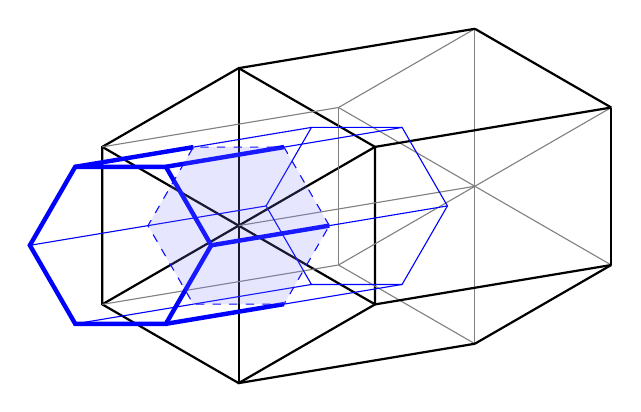
\begin{tikzpicture}
\def\primalstyle{thick}
\def\dualstyle{thick}
\coordinate (P0) at (0cm, 0cm);
\foreach \i in {1,2,...,6}
{
\coordinate (P\i) at ({60*\i-30}:2cm);
\draw[\primalstyle] (P0) -- (P\i);
}
\draw[\primalstyle] (P1) -- (P2) -- (P3) -- (P4) -- (P5) -- (P6) -- cycle;
\begin{scope}[shift={(3cm,0.5cm)}]
    \coordinate (PP0) at (0cm, 0cm);
    \foreach \i in {1,2,...,6}
    {
    \coordinate (PP\i) at ({60*\i-30}:2cm);
    \draw[gray] (PP0) -- (PP\i);
    }
\end{scope}

\draw[\primalstyle] (PP1) -- (PP2);
\draw[gray] (PP2) -- (PP3);
\draw[gray] (PP3) -- (PP4);
\draw[gray] (PP4) -- (PP5);
\draw[\primalstyle] (PP5) -- (PP6);
\draw[\primalstyle] (PP6) -- (PP1);

\draw[gray] (P0) -- (PP0);
\draw[\primalstyle] (P1) -- (PP1);
\draw[\primalstyle] (P2) -- (PP2);
\draw[gray] (P3) -- (PP3);
\draw[gray] (P4) -- (PP4);
\draw[\primalstyle] (P5) -- (PP5);
\draw[\primalstyle] (P6) -- (PP6);

\foreach \i in {1,2,...,6}
{
\coordinate (D\i) at ({60*\i-60}:{2./1.737});
}
\draw[dashed, blue] (D1) -- (D2) -- (D3) -- (D4) -- (D5) -- (D6) -- cycle;
\begin{scope}[shift={(1.5,0.25)}]
    \foreach \i in {1,2,...,6}
    {
    \coordinate (DD\i) at ({60*\i-60}:{2./1.737});
    }
\end{scope}
\draw[blue] (DD1) -- (DD2) -- (DD3) -- (DD4) -- (DD5) -- (DD6) -- cycle;
\draw[blue] (D1) -- (DD1);
\draw[blue] (D2) -- (DD2);
\draw[blue] (D3) -- (DD3);
\draw[blue] (D4) -- (DD4);
\draw[blue] (D5) -- (DD5);
\draw[blue] (D6) -- (DD6);

\begin{scope}[shift={(-1.5,-0.25)}]
    \foreach \i in {1,2,...,6}
    {
    \coordinate (DDD\i) at ({60*\i-60}:{2./1.737});
    }
\end{scope}
\draw[blue, ultra thick] (DDD1) -- (DDD2) -- (DDD3) -- (DDD4) -- (DDD5) -- (DDD6) -- cycle;
\draw[blue, ultra thick] (D1) -- (DDD1);
\draw[blue, ultra thick] (D2) -- (DDD2);
\draw[blue, ultra thick] (D3) -- (DDD3);
\draw[blue] (D4) -- (DDD4);
\draw[blue] (D5) -- (DDD5);
\draw[blue, ultra thick] (D6) -- (DDD6);

\fill[blue!50, opacity=0.2] (D1) -- (D2) -- (D3) -- (D4) -- (D5) -- (D6);

\end{tikzpicture}

\begin{align}
    &\oint_{\partial A} \mathbf{E} \cdot d\mathbf{s} \ = - \iint_A \frac{\partial \mathbf{B}}{\partial t} \cdot d\mathbf{A}, \label{equ:maxwell_int_faraday}\\
    &\oint_{\partial A} \mathbf{H} \cdot d\mathbf{s} \ = \iint_A \left(\frac{\partial \mathbf{D}}{\partial t} + \mathbf{J}\right) \cdot d\mathbf{A}, \label{equ:maxwell_int_ampere}\\
    &\oint_{\partial V} \mathbf{B} \cdot d\mathbf{A} = 0, \label{equ:maxwell_int_gauss_B}\\
\end{align}

\end{document}